\documentclass[11pt]{article}
\usepackage{amsmath, bm}
\usepackage{ntheorem}
\usepackage{fullpage}
\usepackage{amsfonts}
\usepackage{setspace}
\usepackage{graphicx}
\usepackage{ctex}
\usepackage[section]{placeins} %Force figures in the same section
\usepackage{fullpage}
%\usepackage{titlesec} 

%\newcommand{\mycmd}[2]{$\mathbb{#1}^{#2}$} falied to perform

%\theorembodyfont{\normalfont}
%\newtheorem*{definition*}{Definition}
%
\theorembodyfont{\normalfont}
\newtheorem{remark}{Remark}
%
%\theorembodyfont{\normalfont}
%\newtheorem*{errata*}{Errata}
%
\theorembodyfont{\normalfont}
\newtheorem{question}{Question}

\newcommand{\divergence}{\nabla\cdot}
\newcommand{\bmv}{\bm{v}}
%
%\theorembodyfont{\normalfont}
%\newtheorem{theorem}{Theorem}
%
%\theorembodyfont{\normalfont}
%\newtheorem*{proposition*}{Proposition}
%
%\newcommand{\ind}[1][17]{\setlength{\parindent}{#1pt}} % Create an indentation of length 17pt

%\usepackage{mathrsfs} % 6 maths fonts

%\titlespacing{\section}{0pt}{20pt}{20pt}
\title{笔试答卷}
\author{侯怡枫}
%\date{}
%\doublespacing
\onehalfspacing
\newcounter{mycount}




\begin{document}

\maketitle

答卷中用到的源代码都将在Email附件中附上。所有程序都在Linux Ubuntu LTS 16.04操作系统上编译。

\section*{第1题}

这一题的源代码在ans1.R文件中。首先用R将数据绘图获得一个直观的感受。
\begin{figure}[h]
	\centering
	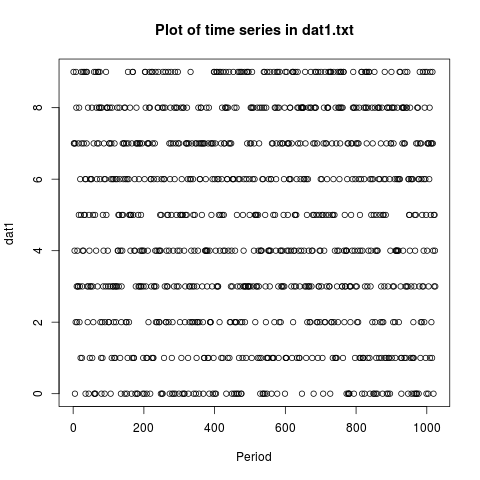
\includegraphics[scale=0.4]{dat1_plot.png}
	\caption{dat1.txt 中数据的时间序列图}
\label{dat1_plot}
\end{figure}

根据图\ref{dat1_plot}, 改时间序列并不呈现确定性时间趋势(deterministic time trend)。然后,图\ref{dat1_acf} 展示改题数据的样本ACF。 图\ref{dat1_pacf}展示改题数据的样本PACF。

\begin{figure}[h]
	\centering
	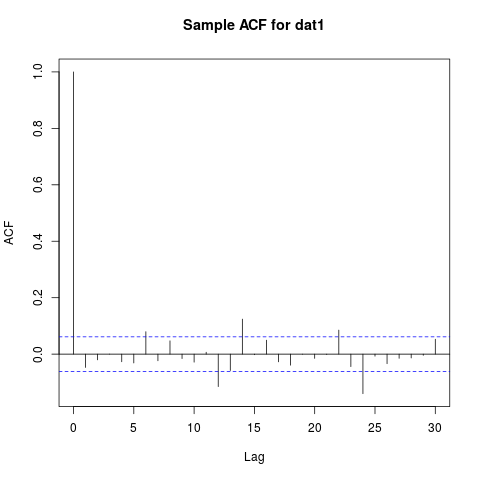
\includegraphics[scale=0.4]{dat1_acf.png}
	\caption{dat1.txt 中数据的样本ACF plot}
\label{dat1_acf}
\end{figure}

\begin{figure}[h]
	\centering
	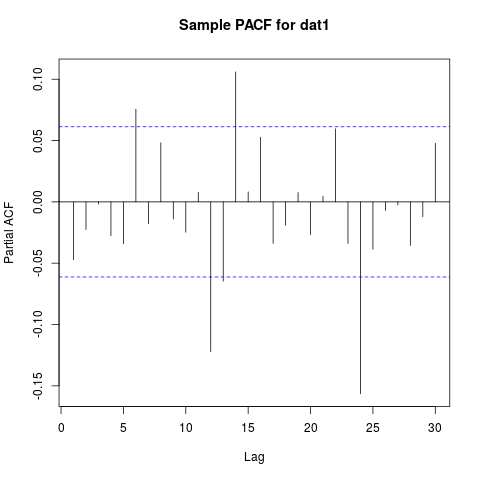
\includegraphics[scale=0.4]{dat1_pacf.png}
	\caption{dat1.txt 中数据的样本PACF plot}
\label{dat1_pacf}
\end{figure}

从图\ref{dat1_acf}中可以看到,该序列和$k=1$的滞后项的样本相关系数接近1。而大于1的滞后项的相关系数则呈指数化递减。从图\ref{dat1_pacf}中可以看到,偏自相关函数在0附近浮动。 这显示此序列可能由一个自回归(AR)过程产生。

答题者选择“存在单位根”作为原假设。相应的备择假设是“产生改序列的随机过 程是平稳的”。答题者计划使用ADF(augmented Dickey-Fuller)检验。这里假设该序列是由一个自回归(AR)模型产生。为使用ADF检验,首先要选择一个信息标准(Information Criterion)来确定自回归的滞后步长(lag)。这里答题者选择AIC进行模型选择。对本题时间序列运行AIC后确定的滞后步长是24。

在确定滞后步长后,运行ADF检验后得到的Dickey-Fuller统计值是-7.6675,对应的$p$值小于0.01。所以结论是拒绝“存在单位根的原假设”。单位根检验在金融时间序列分析和量化投资中非常重要。\textbf{统计套利}这一类策略成功的前提假设是金融资产的价格倾向于回归到均值。但是对一个存在单位根的价格序列来说这个前提是不成立的。


\section*{第四题}
本题涉及的代码在“ans4.r”文件中。

Hurst是用来度量时间序列的长期记忆性。Hurst指数的值在0.5到1之间意味着长期的正相关性,简单来说意味着序列中一个较高的值往往会跟随者另一个较高的值。Hurst指数的值在0到0.5之间意味着长期的负相关性。Hurst指数的值等于0.5则意味着一个完全不相关的序列。Hurst指数的定义如下:
\begin{equation}
E\bigg[\frac{R(n)}{S(b)}\bigg]=Cn^H,\ n \rightarrow \infty
\end{equation}
其中$R(n)$是前$n$个值的值域,$S(n)$是标准差,$E[x]$是期望值,$n$是观察的期数,$C$是一个常数。对本题上证指数序列,答题者使用R/S方法进行参数估计和假设检验。首先假设整个序列的观察数量是$N$,将其等分为每个长度为$n$的子区间。定义$A$为$\frac{N}{n}$的整数部分,也就是子区间的数量。具体方法如下,(参考\cite{Qian2004}):

1. 计算均值:
\begin{equation}
m=\frac{1}{n}\sum\limits_{i=1}^{n}X_i
\end{equation}

2. 计算均值调整后的序列:
\begin{equation}
Y_t = X_t -m, \ \ t=1,2,...n
\end{equation}

3. 计算累计偏离序列:
\begin{equation}
Z_t = \sum\limits_{i=1}^{t} Y_i, \ \ t=1,2,...,n
\end{equation}

4. 计算值域$R$:
\begin{equation}
R(n) = \text{max}(Z_1,Z_2,...,Z_n)-\text{min}(Z_1,Z_2,...,Z_n)
\end{equation}

5. 计算标准差$S$:
\begin{equation}
S(n)=\sqrt{\frac{1}{n}\sum\limits_{i=1}^n(X_i-m)^2}
\end{equation}

6. 计算每一个子区间的$R(n)/S(n)$值并求平均。

7. 最后把$\text{log}(n)$作为控制变量,$\text{log}[ R(n)/S(n)]$ 作为应变量进行线性回归,估计斜率并进行假设检验。 这里的log函数定义为以2为底。

首先,仅仅是为了简化计算,这里采用最近的4096($2^{12}$)天的收盘价数据作为观察样本。 将$N=4096$个数据划等分分成$2,4,...,2048$ 个区间。对每一种划分使用如上算法计算出$R(n)/S(n)$(作为$n$的函数)的值并绘图,见图\ref{logRS}
\begin{figure}[h]
	\centering
	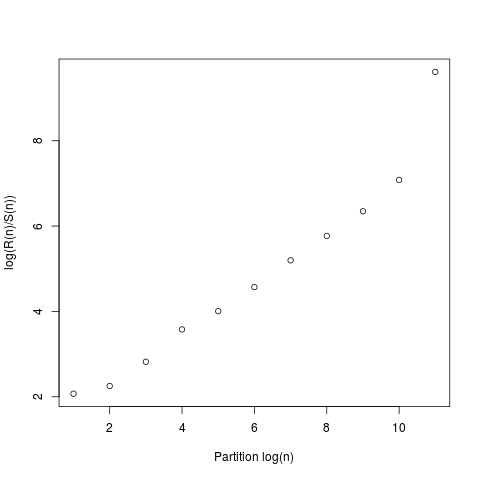
\includegraphics[scale=0.4]{logRS.png}
	\caption{$\text{log}\frac{R(n)}{S(n)}$}
\label{logRS}
\end{figure}

用OLS估计出的斜率($H$值)为0.71771(长期正相关)。对于统计检验我们选择“$H=0.5$ (没有长期相关性)”作为原假设。计算的$p$值为1.633015e-05。误差项的有限分布的推到是一件非常困难的工作,具体可参考文献。所以这里的假设检验的前提是回归的误差项是正态分布的。


\bibliographystyle{plain}
\bibliography{Tornado}

\end{document}